\section{实验}
\label{sec:experiments}

我们分别评估两项操作：在历史不断增长且身份可修订的情况下保存记录，以及针对问题读取所需的证据。

\subsection{评估设置}
\label{sec:setup}

我们使用四个公开基准。主要的MemoryAgentBench（MAB）评估包含10个任务组、59份文档和767道配对题；Align+扩展到14个任务组、1{,}074道题（完整集合为29个任务组、3{,}671道题）。所有MAB分数均由官方评分器\footnote{本轮实验固定使用提交\texttt{455306d}的评分器。}计算，回答模型为Kimi-K3。LongMemEval先写入完整对话集合，再用配对的$n{=}25/25/27$样本运行三种回答方法。MAB以百分比报告（100表示全部正确，0表示全部错误）；AR为\emph{Accurate Retrieval}，TTL为\emph{Test-Time Learning}，LRU为\emph{Long-Range Understanding}，SF为\emph{Selective Forgetting}；MCC为\emph{Multi-Class Classification}，Recom为按Recall@5评分的电影推荐，FC-SH/FC-MH分别为单跳和多跳FactConsolidation。Recall、$J$、exact-match和Overall均为越高越好，calls、tokens和bytes为成本指标。采样与评审细节见附录~\ref{app:sampling}，附录表~\ref{tab:experiment-map}说明各基准对应存储问题还是读取问题。

\begin{figure*}[t]
  \centering
  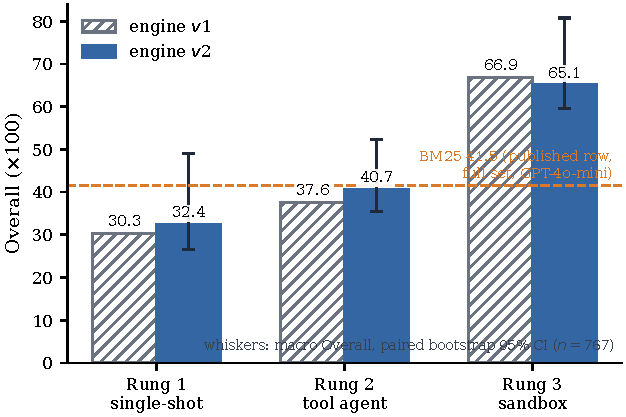
\includegraphics[width=\textwidth]{figures/fig2_ladder.pdf}
  \caption{MemoryAgentBench results by method and task (official scorer, Kimi-K3 answerer). (a) Overall scores: Base on the frozen paired sample ($n{=}767$), Align+ on the extended sample ($n{=}1074$), with marginal 95\% bootstrap intervals; (b) Align+ domain scores at the extended sample; (c) selected task scores; (d) all 209 residual zero-score items of the extended sample. The two sample definitions are labeled separately.}
  \label{fig:ladder}
\end{figure*}

\subsection{如何存储：更新与实体对齐}
\label{sec:temporal-benchmark}
\label{sec:engine-versions}
\label{sec:engine-paired}
\label{sec:deletion-boundary}

LongMemEval检验完整对话历史写入后，早期陈述和后续修正是否都能被找到。在配对运行中，直接检索由0.68升至0.72，记忆工具阅读由0.68升至0.72，原文支撑阅读由0.889升至0.926（$n{=}25/25/27$；这些轨迹样本较小，只能作方向性观察）。这些配对运行表明，新旧观测可以由同一读取路径共同访问。独立的500题LongMemEval-S运行达到84.60\%，回答者和评审均为Qwen3.7-plus；该协议与表中其他回答者/评审组合不同。

对齐实验检验身份何时被最终确定。即时对齐逐窗口决策，延迟对齐则等待周围证据。在配对写入记录中，每份MAB文档的调用由609降至329，每份LongMemEval文档由63.8降至22.0。同名重复族在MAB上由340降至124，在LongMemEval上由482降至99。配对样本中MCC和FC-MH各提高3个百分点，95\%区间为$-7$至$+13$（包含零）。这些数据对应一个组合式写入路径，其中同时使用延迟对齐、批处理和并发处理；实际效果是降低构建成本，并为修订身份链接提供更多机会。三臂分解见附录表~\ref{tab:alignment-ab}，附录图~\ref{fig:alignment-outcomes}分别展示成本、重复族和质量变化。

MEME把历史保留与删除区分开来：100个episode共进行694次后任务检查，删除准确率为0\%，级联为46.34\%，缺失为59.23\%。这个零值是当前写入/读取路径的属性：MEME删除事件要求系统停止返回某条旧事实，同时保留周围历史；测试路径却把删除陈述记录为另一条观测，没有墓碑标记，也没有从实体或关系传播到受影响片段的查询时抑制规则，因此证据虽被保留，仍会被检索。支持删除需要记录删除目标，把不可用状态传播到派生指针，并区分当前查询与历史查询。这个结果精确定位了缺失操作，不能说明仅靠保留来源就实现了遗忘。对应的更新、邻居跳转和删除分解见附录图~\ref{fig:diagnostics}。

\subsection{如何读取：渐进式证据检索}
\label{sec:ladder}
\label{sec:relational-benchmark}

图~\ref{fig:ladder}给出分面板结果。面板(a)在Align+上约由33升至40再升至71；面板(b)显示原文路径达到88.8 AR、52.9 TTL、62.3 LRU和80.0 SF，而其他路径的TTL仍为2.6。面板(c)在MCC（46.0）和FC-MH（70.0）上呈现相同优势；面板(d)显示209道零分题中有122道属于TTL。因而，增益与原文访问以及围绕更新和事实整合的持续取证有关。

三条路径（\cref{sec:answer-paths}）在答案者获得的内容和追加请求的权限上不同。\textbf{固定检索}一次性生成记忆记录和分块的排序列表，不能修改、重新打开或核对。\textbf{记忆工具阅读}可以多次发起只读调用，第二次调用可利用第一次返回的实体或关系，但答案者的上下文局限于工具返回的记录，没有来源文件门。\textbf{原文支撑阅读}用同一索引选择文档组，再打开原始文件，只把通过来源门的片段交给答案者。因此，第二条路径是在存储记录上的自适应导航，第三条路径则在此基础上增加原文阅读。

逐行结果呈现相同模式：原文阅读在MCC、FC-MH、MH-QA和LongMemEval-S上最强，而工具阅读主要帮助DetectiveQA等任务。这些任务中，第一段看似相关的分块并不够用，智能体必须合并多次提及、追踪更新或核对限定词。固定路径无法请求缺失提及；工具路径可以请求另一条有界记录；原文路径能够检查所选文件并核对措辞。614题热图和路径协议对比见附录图~\ref{fig:alignment}与附录表~\ref{tab:answer-path-differences}。

全文参考在文档组适合预算的614道题上达到78.7。原文支撑阅读在相同题目上为70.8，在扩展的1{,}074题上为71.0，并且仍可处理超出预算的460道题。全文上下文在能够容纳时表现很强，而地址化读取可以在语料超过单一窗口后继续工作。

LoCoMo在Mem0兼容的二元$J$指标下测试跨Episode证据（即由语言模型评审判定为正确的答案比例）。Deep-Dream总体达到95.19\%（单跳97.38，多跳93.62，开放域80.21，时间95.33），独立的Qwen3.7-plus交叉评审在同一答案上给出94.22\%。由于1,540行中有1,529行早于运行时代码指纹记录，我们将其作为单次诊断；已发表的Mem0和Zep行保留各自的回答者、评审者和测试流程。多跳与时间结果与设计相符：关系路径连接Episode，来源观测保留支撑陈述。

\begin{table*}[t]
\centering
\footnotesize
\setlength{\tabcolsep}{4.5pt}
\renewcommand{\arraystretch}{1.12}
\begin{tabular*}{\textwidth}{@{\extracolsep{\fill}}lrrrrrrr@{}}
\toprule
 & \multicolumn{2}{c}{Direct retrieval}
 & \multicolumn{2}{c}{Tool-assisted reading}
 & \multicolumn{2}{c}{Source reading}
 & \multicolumn{1}{c}{\shortstack{Source$-$Direct\\(Align+)}} \\
\cmidrule(lr){2-3}\cmidrule(lr){4-5}\cmidrule(lr){6-7}\cmidrule(lr){8-8}
Task / domain
 & Base & Align+ & Base & Align+ & Base & Align+
 & \shortstack{Source$-$Direct\\(Align+)} \\
\midrule
\rowcolor{blue!10}
\multicolumn{8}{@{}l}{\textbf{AR: Accurate Retrieval}} \\
SH-QA
 & 54.0 & 48.0 & 84.0 & 72.0 & \textbf{94.0} & \underline{92.0} & 44.0 \\
MH-QA$^{\ddagger}$
 & -- & 22.0 & -- & \underline{42.0} & -- & \textbf{77.0} & 55.0 \\
LongMemEval-S$^{*}$
 & 26.7 & 41.7 & 43.3 & 51.7 & \textbf{90.0} & \underline{88.3} & 46.6 \\
EventQA
 & \underline{90.3} & 89.7 & \underline{90.7} & 88.3 & \textbf{98.0} & \textbf{98.0} & 8.3 \\
\midrule
\rowcolor{green!10}
\multicolumn{8}{@{}l}{\textbf{TTL: Temporal and Test-time Learning}} \\
MCC, icl\_clinic150
 & 4.0 & 2.0 & 3.0 & 2.0 & \underline{43.0} & \textbf{46.0} & 44.0 \\
Recom$^{\ddagger}$
 & -- & \underline{3.2} & -- & \underline{3.2} & -- & \textbf{59.8} & 56.6 \\
\midrule
\rowcolor{orange!12}
\multicolumn{8}{@{}l}{\textbf{LRU: Long-range Understanding}} \\
$\infty$Bench-Sum$^{\dagger}$
 & 0.0 & 0.0 & \underline{28.4} & \textbf{29.8} & 21.2 & 0.0 & 0.0 \\
DetectiveQA
 & 50.0 & \underline{66.7} & 50.0 & \textbf{83.3} & \textbf{83.3} & \textbf{83.3} & 16.6 \\
\midrule
\rowcolor{purple!10}
\multicolumn{8}{@{}l}{\textbf{SF: Selective Forgetting}} \\
FC-SH
 & \underline{68.0} & 66.0 & 67.0 & 63.0 & \textbf{90.0} & \textbf{90.0} & 24.0 \\
FC-MH
 & 2.0 & 3.0 & 4.0 & 4.0 & \underline{67.0} & \textbf{70.0} & 67.0 \\
\midrule
\rowcolor{gray!12}
\textbf{Overall ($n=767$)}
 & 30.2 & 32.4 & 37.6 & 40.7 & \textbf{66.9} & \underline{65.1} & 32.7 \\
Overall ($n{=}1074$, extended)
 & -- & 33.3 & -- & 40.0 & -- & \textbf{71.0} & 37.7 \\
\bottomrule
\end{tabular*}
\caption{MemoryAgentBench scores (percent). The last column is Source$-$Direct within Align+; it is reported when both Align+ paths are available. Bold and underlining mark the best and second-best entry within each row.}
\label{tab:main-results}
\end{table*}



\begin{figure*}[t]
  \centering
  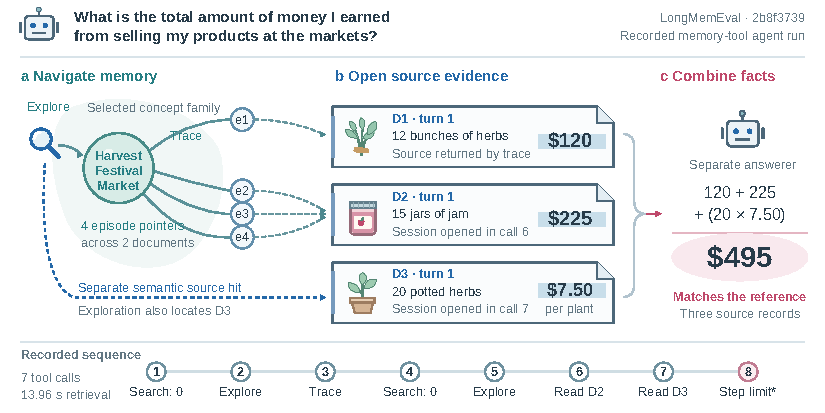
\includegraphics[width=0.88\textwidth]{figures/fig4_agent_trace.pdf}
  \caption{Recorded LongMemEval trace (question \texttt{2b8f3739}): concept tracing exposes four episode pointers across two documents, and semantic retrieval locates the third sales record. Seven successful calls read $120$, $225$, and $7.50$; a malformed eighth response reaches the step limit, after which a separate answerer computes $495$. The trace shows graph navigation locating candidates and source spans supplying the arithmetic.}
  \label{fig:agent-trace}
\end{figure*}


一个实际的LongMemEval轨迹具体展示了存储结构和读取过程如何衔接。智能体先沿着概念和关系指针跨越两份文档，再打开包含\$120、\$225、数量20和单价\$7.50的原文片段，计算出$120+225+(20\times7.50)=495$。七次成功调用显示图结构负责定位候选，原文片段提供算术所需的数值；第八次格式错误并达到步数上限的记录也被保留，便于审计。这个案例用于说明读取过程，不替代总体基准结果。

\subsection{与现有记忆系统的比较}
\label{sec:cross-system}

表~\ref{tab:main-cross-system}将Deep-Dream与MAB、LoCoMo和LongMemEval-S的已发表结果并列，模型列明确每种配对。在MAB行中固定使用Kimi-K3：固定检索33.3，迭代记忆工具40.0，原文阅读71.0；78.7的全文行是在文档适合窗口的614道题上的同模型参考上限。已发表行保留其原有回答者和评审者，因此只有同模型MAB配对构成受控比较。分类复现见附录表~\ref{tab:mem0-baselines}--\ref{tab:zep-longmemeval}和~\ref{tab:mem0-f1-bleu}。绿色行标记近期强模型报告：$\dagger$使用GPT-5-mini/GPT-5，$\ddagger$使用GPT-4.1-mini或GPT-5-mini并由GPT-4o-mini评审，$\ast$使用Gemini-3 Pro以及GPT-OSS-120B记忆和评审\citep{ji2026infini,wang2026memmachine,latimer2025hindsight}。LongMemEval-S上，Deep-Dream的84.6（Qwen3.7-plus回答者和评审者）低于MemMachine（93.0）、Hindsight（91.4）和Supermemory（85.2）；差距主要集中在会话偏好、时间推理和多会话问题。Deep-Dream在助手事实、用户事实和知识更新上较强；这些是下一步读取和更新的目标，同时保留MAB上的原文读取优势以及LoCoMo多跳和时间维度的表现。

对于Infini Memory-A，MAB行采用其论文报告的四类平均值：AR为81.2，TTL为51.0，LRU为68.6，SF为58.0，总体为64.7；不以更细的子任务分数替换这些类别值。

\begin{table*}[t]
\centering
\scriptsize
\setlength{\tabcolsep}{2.4pt}
\renewcommand{\arraystretch}{0.82}
{\footnotesize\textbf{(a) MemoryAgentBench (official scorer)}}\\[1.5pt]
\begin{tabular*}{\textwidth}{@{\extracolsep{\fill}}>{\raggedright\arraybackslash}p{0.25\textwidth}>{\raggedright\arraybackslash}p{0.15\textwidth}rrrrr@{}}
\toprule
Memory system & Answerer & AR & TTL & LRU & SF & Overall \\
\midrule
Full context & GPT-4o & 58.1 & 50.0 & 54.9 & 32.5 & 48.8 \\
Full context & GPT-4o-mini & 49.2 & 48.6 & 46.2 & 25.0 & 42.2 \\
Full context & GPT-4.1-mini & 71.8 & 46.2 & 49.1 & 20.5 & 46.9 \\
Full context & Gemini-2.0-Flash & 65.1 & 46.4 & 41.6 & 16.5 & 42.4 \\
Full context & Claude-3.7-Sonnet & 59.7 & 53.9 & 62.2 & 22.5 & 49.6 \\
\rowcolor{blue!9}
Full context ($n{=}614$) & Kimi-K3 & \textbf{96.8} & \textbf{75.0} & 65.2 & 78.0 & \textbf{78.7} \\
\midrule
BM25 RAG & GPT-4o-mini & 60.5 & 44.5 & 35.6 & 25.5 & 41.5 \\
HippoRAG-2 & GPT-4o-mini & 65.1 & 35.8 & 36.2 & 29.5 & 41.6 \\
MIRIX & GPT-4.1-mini & 63.0 & 35.7 & 40.5 & 11.5 & 37.7 \\
MemGPT & GPT-4o-mini & 34.3 & 40.8 & 22.4 & 15.5 & 28.3 \\
Zep & GPT-4o-mini & 37.5 & 37.5 & 16.2 & 5.0 & 24.0 \\
Mem0 & GPT-4o-mini & 32.6 & 21.2 & 20.7 & 10.0 & 21.1 \\
\rowcolor{green!9}
Infini Memory-A & GPT-5-mini$^\dagger$ & 81.2 & 51.0 & \textbf{68.6} & 58.0 & 64.7 \\
\midrule
\rowcolor{blue!9}
Deep-Dream / Direct retrieval & Kimi-K3 & 50.3 & 2.6 & 45.9 & 34.5 & 33.3 \\
\rowcolor{blue!9}
Deep-Dream / Memory-tool agent & Kimi-K3 & 63.5 & 2.6 & 60.4 & 33.5 & 40.0 \\
\rowcolor{blue!9}
\textbf{Deep-Dream / Source reading} & \textbf{Kimi-K3} & 88.8 & 52.9 & 62.3 & \textbf{80.0} & 71.0 \\
\bottomrule
\end{tabular*}

\vspace{3pt}
{\footnotesize\textbf{(b) LoCoMo $J$ score (\%; Mem0 scoring)}}\\[1.5pt]
\begin{tabular*}{\textwidth}{@{\extracolsep{\fill}}>{\raggedright\arraybackslash}p{0.25\textwidth}>{\raggedright\arraybackslash}p{0.15\textwidth}rrrrr@{}}
\toprule
Memory system & Answerer / judge & Single-hop & Multi-hop & Open-domain & Temporal & Weighted \\
\midrule
Mem0 & GPT-4o-mini & 67.13 & 51.15 & 72.93 & 55.51 & $\approx$62.14 \\
Mem0$^g$ & GPT-4o-mini & 65.71 & 47.19 & 75.71 & 58.13 & $\approx$61.36 \\
Zep & GPT-4o-mini & 61.70 & 41.35 & 76.60 & 49.31 & $\approx$56.32 \\
LangMem & GPT-4o-mini & 62.23 & 47.92 & 71.12 & 23.43 & $\approx$52.08 \\
OpenAI & GPT-4o-mini & 63.79 & 42.92 & 62.29 & 21.71 & $\approx$51.10 \\
A-Mem$^*$ & GPT-4o-mini & 39.79 & 18.85 & 54.05 & 49.91 & $\approx$38.95 \\
\midrule
\rowcolor{green!9}
MemMachine & GPT-4.1-mini / GPT-4o-mini$^\ddagger$ & 95.12 & 88.30 & 71.88 & 91.59 & 91.69 \\
\rowcolor{green!9}
Hindsight & Gemini-3 Pro / GPT-OSS-120B$^\ast$ & 86.17 & 70.83 & \textbf{95.12} & 83.80 & 89.61 \\
\midrule
\rowcolor{blue!9}
Deep-Dream (diagnostic) & Kimi-K3 & 97.38 & 93.62 & 80.21 & 95.33 & 95.19 \\
\rowcolor{blue!9}
Deep-Dream & Qwen3.7-plus / Qwen3.7-plus & 96.91 & 92.91 & 77.08 & 93.46 & 94.22 \\
\bottomrule
\end{tabular*}

\vspace{3pt}
{\footnotesize\textbf{(c) LongMemEval-S (\%)}}\\[1.5pt]
{\tiny\setlength{\tabcolsep}{0pt}\begin{tabular*}{\textwidth}{@{\extracolsep{\fill}}>{\raggedright\arraybackslash}p{0.25\textwidth}>{\raggedright\arraybackslash}p{0.15\textwidth}rrrrrrr@{}}
\toprule
Memory system & Answerer / judge & Overall & Sess. pref. & Sess. asst. & Temporal & Multi-sess. & Knowl. upd. & Sess. user \\
\midrule
Full context & GPT-4o-mini & 55.4 & 30.0 & 81.8 & 36.5 & 40.6 & 76.9 & 81.4 \\
Full context & GPT-4o & 60.2 & 20.0 & 94.6 & 45.1 & 44.3 & 78.2 & 81.4 \\
\midrule
Zep & GPT-4o-mini & 63.8 & 53.3 & 75.0 & 54.1 & 47.4 & 74.4 & 92.9 \\
Zep & GPT-4o & 71.2 & 56.7 & 80.4 & 62.4 & 57.9 & 83.3 & 92.9 \\
\rowcolor{green!9}
MemMachine & GPT-5-mini$^\ddagger$ & \textbf{93.0} & \textbf{93.3} & 98.2 & \textbf{91.7} & \textbf{87.2} & \textbf{94.9} & \textbf{100.0} \\
\rowcolor{green!9}
Hindsight & Gemini-3 Pro$^\ast$ & 91.4 & 80.0 & 96.4 & 91.0 & \textbf{87.2} & \textbf{94.9} & 97.1 \\
\rowcolor{green!9}
Supermemory & Gemini-3 Pro$^\ast$ & 85.2 & 70.0 & 98.2 & 82.0 & 76.7 & 89.7 & 98.6 \\
\midrule
\rowcolor{blue!9}
\textbf{Deep-Dream} & \textbf{Qwen3.7-plus / Qwen3.7-plus} & 84.6 & 53.3 & \textbf{100.0} & 84.2 & 74.4 & 91.0 & 98.6 \\
\bottomrule
\end{tabular*}}
\caption{Results for Deep-Dream and published memory systems on MemoryAgentBench, LoCoMo, and LongMemEval-S. Each row retains its answerer, judge, subset, and evaluation setting. The Deep-Dream LoCoMo row is a single-run diagnostic; its legacy-fingerprint details are in the appendix. Bold marks each column's maximum among the reported comparable rows; the single-run diagnostic row is intentionally unbolded; the Infini Memory-A row uses the category averages reported in its paper.}
\label{tab:main-cross-system}
\end{table*}



现有系统使用不同的记忆对象：抽取的原子记忆（Mem0）、带有效期窗口的情景图（Zep/Graphiti）、段落图（HippoRAG-2）、链接笔记（A-MEM）或类型化模块（MIRIX）。Deep-Dream保持来源片段的权威性，并以概念和关系作为可修订地址，使智能体能够在原始文件中核验多次提及的答案。

\subsection{检索与证据诊断}
\label{sec:external-comparisons}
\label{sec:provenance-ablation}

我们在相同的210道题上重放四种索引：对原始Episode使用关键词（BM25），再依次加入语义链接、图邻居和关系链接。Recall-any@10询问前十项中是否出现至少一条相关项；Recall-all@10询问是否出现全部相关项。Recall-any@10分别为72.38、72.38、71.43和72.38\%；每个配对差异都落在基于同一重放计算的$\pm$2.4个百分点95\% bootstrap等价界内，其他指标也没有稳定变化。因此，重放没有证据表明图链接单独提升离线召回；它只说明离线检索，而在线阶段实际使用了图的导航作用——在原文阅读前选择文档组、版本和关系链接——并未对该作用做消融。

附录图~\ref{fig:cost}报告相应的调用和token成本。原文支撑阅读由于需要核验并扩展证据，调用更多；但在需要多次提及或更新的问题上也产生最强答案。
